\documentclass{beamer}
\usetheme{Montpellier}
\usefonttheme[onlylarge]{structurebold}
\setbeamerfont*{frametitle}{size=\normalsize,series=\bfseries}
\setbeamertemplate{navigation symbols}{}

\useoutertheme{infolines}

\usepackage{mathtools}
\DeclarePairedDelimiter{\ceil}{\lceil}{\rceil}

\usepackage[english]{babel}
\usepackage[latin1]{inputenc}
\usepackage[T1]{fontenc}

\long\def\/*#1*/{}

\title[Unfolding MWIS on PTASGIG]
{
  Unfolding MWIS on PTASGIG
}
\author[Manass�s]
{
  Manass�s~Ferreira\inst{1} \\
  {\scriptsize
  mfer@dcc.ufmg.br
  }
}
\institute[UFMG]
{
  \inst{1}
Dept. of Computer Science\\
Universidade Federal de Minas Gerais (UFMG)\\
Belo Horizonte, Brazil
}
\date[\today]
{ 
  Introduction to Approximation Algorithms - 2014/2\\
  {\scriptsize
  {\bf Instructors}: Olga Goussevskaia {\it and} Antonio Alfredo \\
  \{olga, loureiro\}@dcc.ufmg.br  
  }
}

\begin{document}

  \begin{frame}
    \titlepage
  \end{frame}

  \begin{frame}{Agenda}
    \tableofcontents
  \end{frame}

  \section{Preliminaries}
    \subsection{PTASGIG}
      \begin{frame}{\small Polynomial-Time Algorithm Scheme for Geometric Intersection Graphs}
        $$n^{O(k ^{2})}$$
        $$k > 1$$
        \begin{figure}[h!]
          \centering
            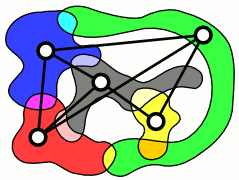
\includegraphics[width=0.50\textwidth]{img/ig.png}
        \end{figure}      
        $$\frac{1}{1+\epsilon} OPT_{IS}(\mathcal{D})$$
        $$\epsilon > 0$$
      \end{frame}

      \begin{frame}{Choosen Paper Cover}
        \begin{figure}[h!]
          \centering
            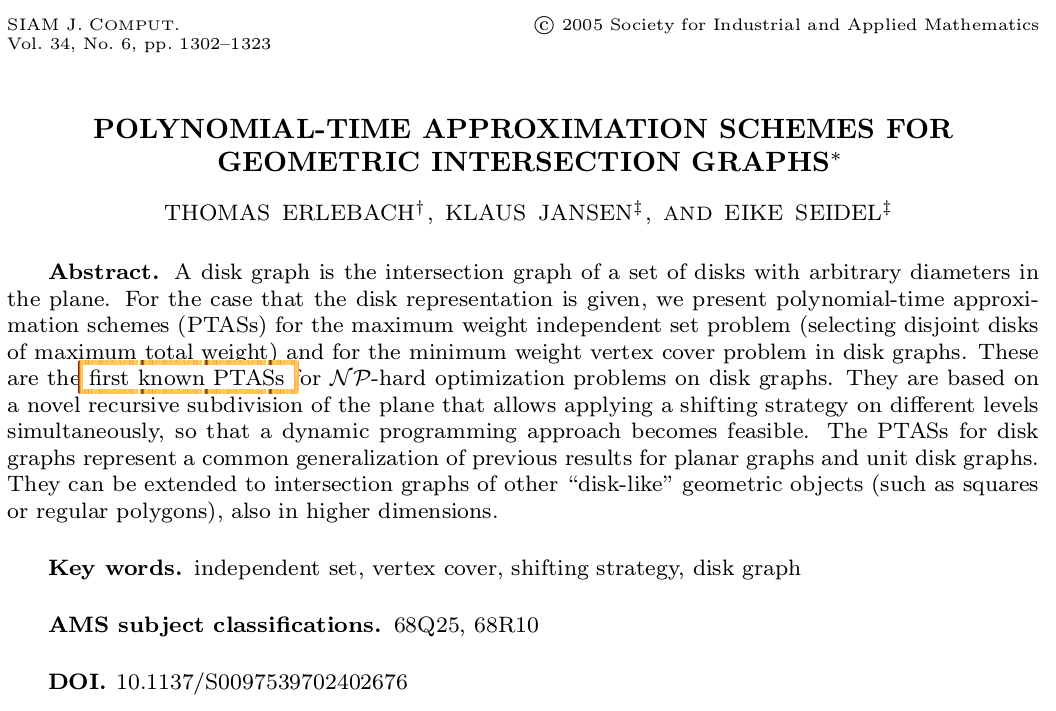
\includegraphics[width=0.9\textwidth]{img/cover.png}
        \end{figure}    
      \end{frame}

      \begin{frame}{Citations at Google Scholar}
        \begin{figure}[h!]
          \centering
            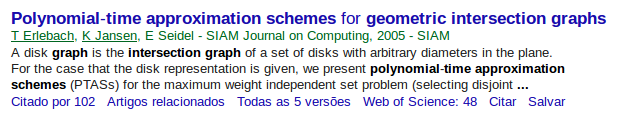
\includegraphics[width=1.0\textwidth]{img/scholar.png}
        \end{figure}    
      \end{frame}

      \begin{frame}{Applications}
        \begin{figure}[h!]
          \centering
            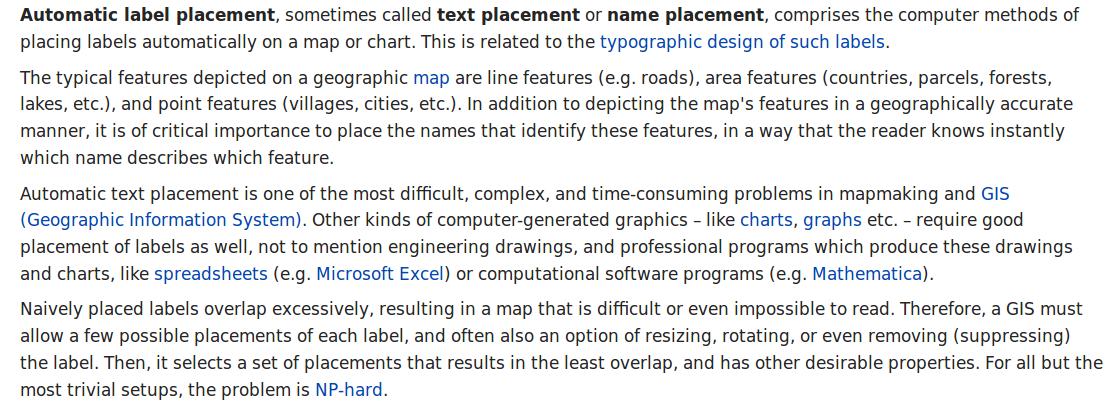
\includegraphics[width=1.0\textwidth]{img/label.png}
        \end{figure}    
        \begin{figure}[h!]
          \centering
            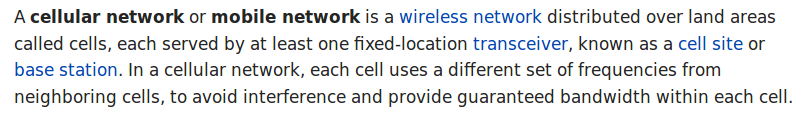
\includegraphics[width=1.0\textwidth]{img/cell-networks.png}
        \end{figure}    
      \end{frame}

      \begin{frame}{Automatic Label Placement}
        \begin{figure}[h!]
          \centering
            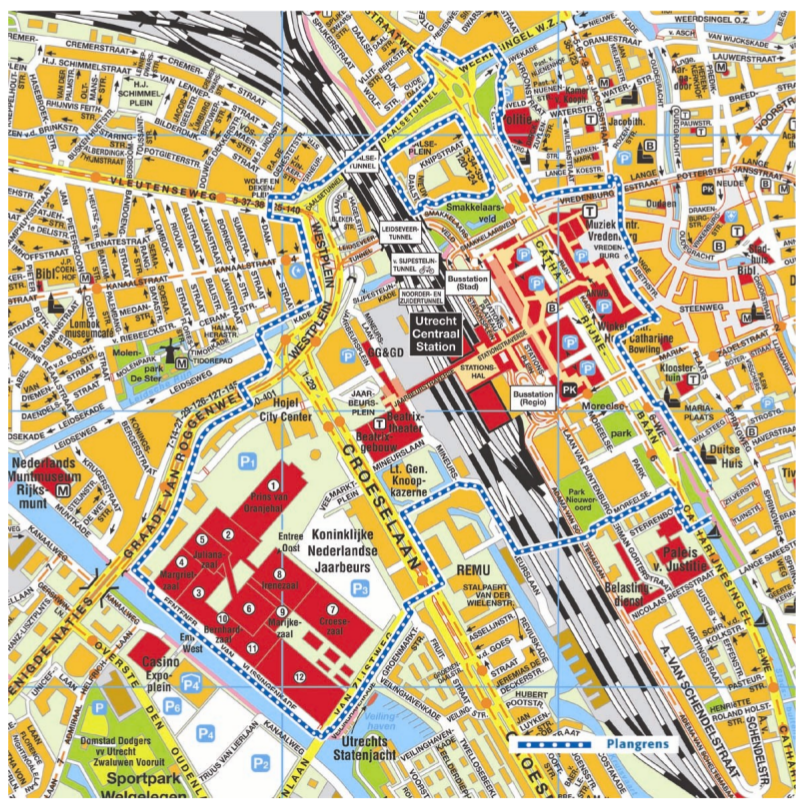
\includegraphics[width=0.5\textwidth]{img/autolabel.png}
        \end{figure}
        Given features on a map and the labels that belong to these features, place the labels near the features without labels
        overlapping other labels or overlapping features on the map
      \end{frame}

      \begin{frame}{Cellular Network}
        \begin{figure}[h!]
          \centering
            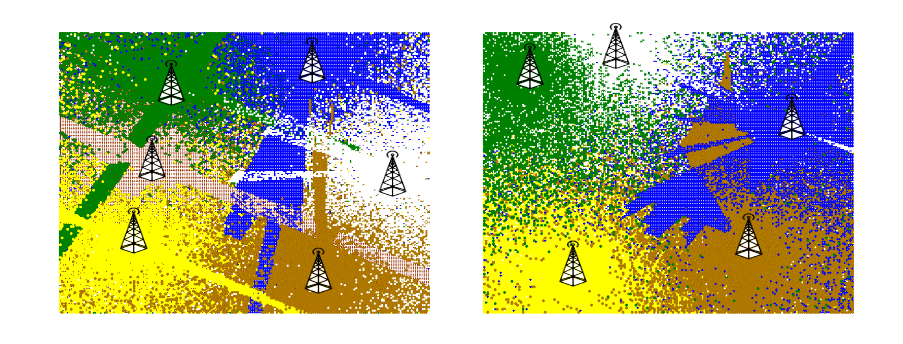
\includegraphics[width=1.0\textwidth]{img/callControl.png}
        \end{figure}    
        The call control problem in a network that supports a spectrum of w available frequencies is to assign frequencies 
        to users so that signal interference is avoided, while maximizing the number of users served.
      \end{frame}

      \begin{frame}{Problems and Results}
        \small PTAS for MWIS and MWVC in the intersection graphs of disks, squares and other {\it disk-like} objects, also in higher dimensions.
        \begin{block}{\small Maximum Weight Independent Set}      
          {\it \tiny The Chosen Problem for this Seminar. Wait for the next slide.} {\color{red}{\Large;}$\land)$}
        \end{block}
        \begin{block}{\small Minimum Weight Vertex Cover}
          Compute a subset of the given objects with minimum total weight such that, 
          for any two intersecting objects, at least one of the objects is contained in the subset.
        \end{block}
      \end{frame}

   \section{Problem Definition}
    \subsection{MWIS}  
      \begin{frame}{Maximum Weight Independent Set}
        \begin{block}{Goal}
          Compute, for a given set of geometric objects with certain weights, 
          a subset of disjoint ({\bf non-overlapping}) objects with maximum total weight.
        \end{block}
        \begin{figure}[h!]
          \centering
          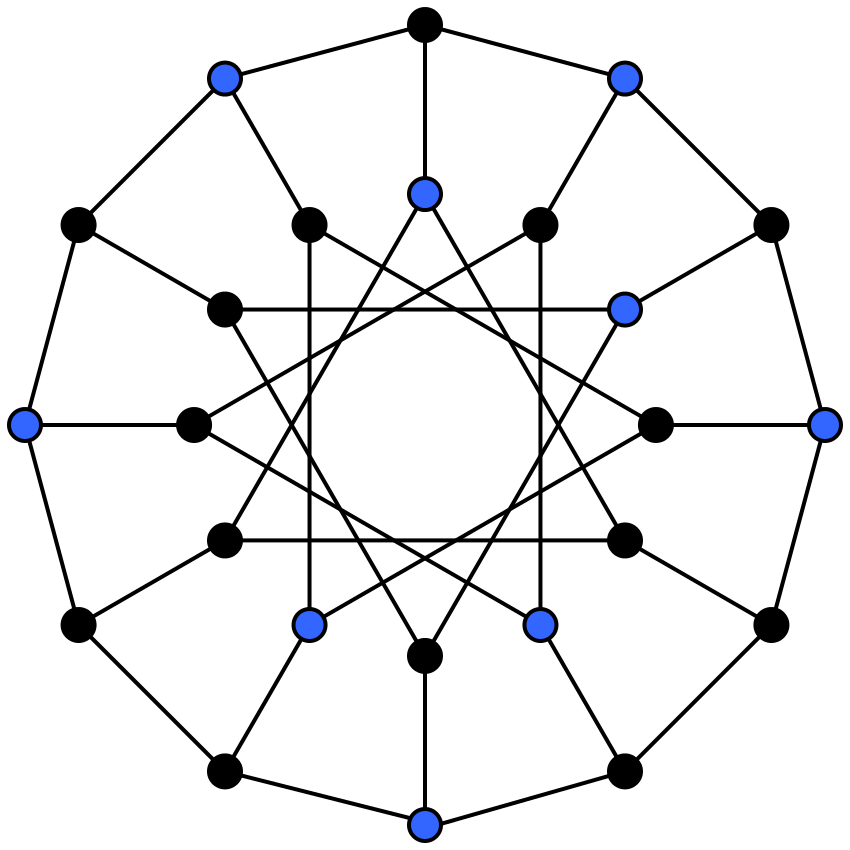
\includegraphics[width=0.4\textwidth]{img/is.png}
          {\tiny Generalized Petersen graph GP(12,4)}
        \end{figure}
      \end{frame}
      \begin{frame}{NP-Completeness}
        \begin{figure}[h!]
          \centering
            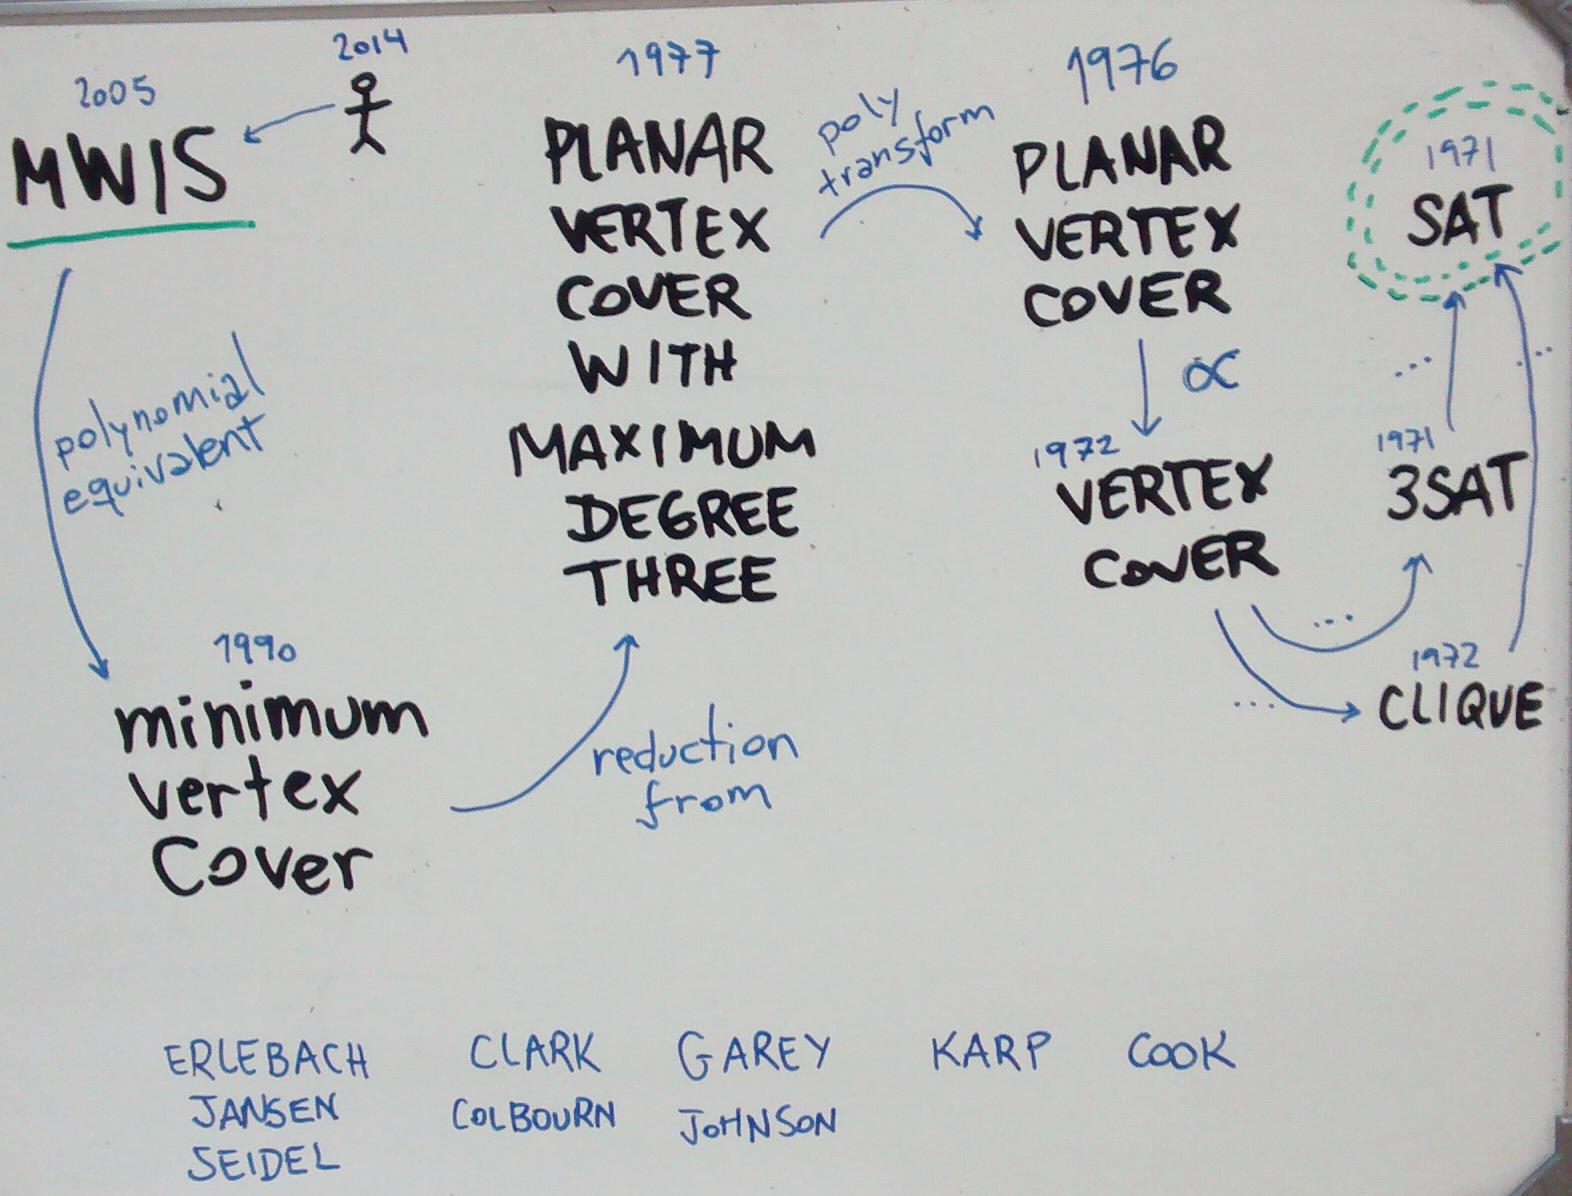
\includegraphics[width=0.8\textwidth]{img/np-hardness-story.png}
        \end{figure}   
      \end{frame}
      
  \section{Model}
    \subsection{Intersection graphs of {\it disk-like objects} }
    \begin{frame}{}
      For a set V of geometric objects, the corresponding intersection graph is the undirected graph with vertex set V and an edge between two vertices if the corresponding objects intersect.
      \begin{figure}[h!]
        \centering
          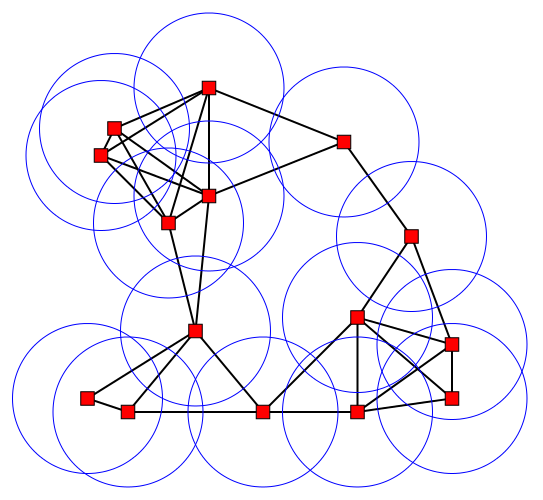
\includegraphics[width=0.50\textwidth]{img/udg.png}
      \end{figure}      
    \end{frame}

    \begin{frame}{}
      \begin{figure}[h!]
        \centering
          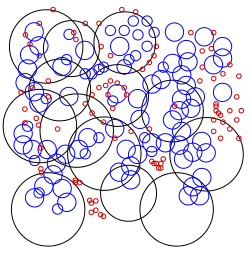
\includegraphics[width=0.255\textwidth]{img/disklike.png}
      \end{figure}    
      \begin{figure}[h!]
        \centering
          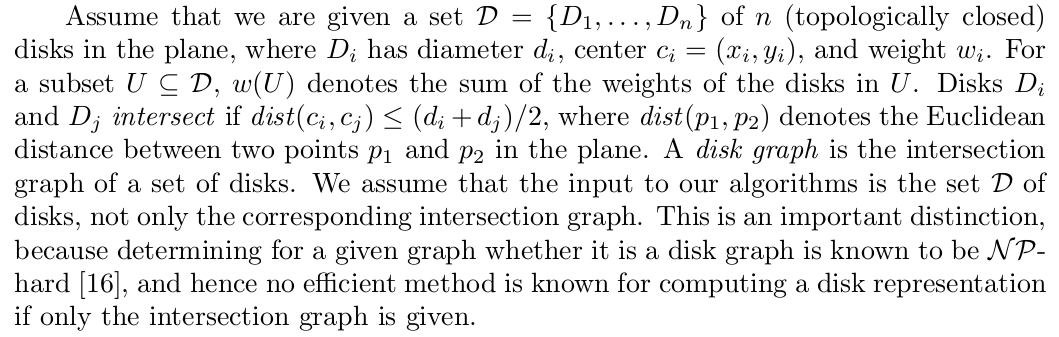
\includegraphics[width=1.0\textwidth]{img/model1.png}
      \end{figure}   
    \end{frame}

    \begin{frame}{}
      \begin{figure}[h!]
        \centering
          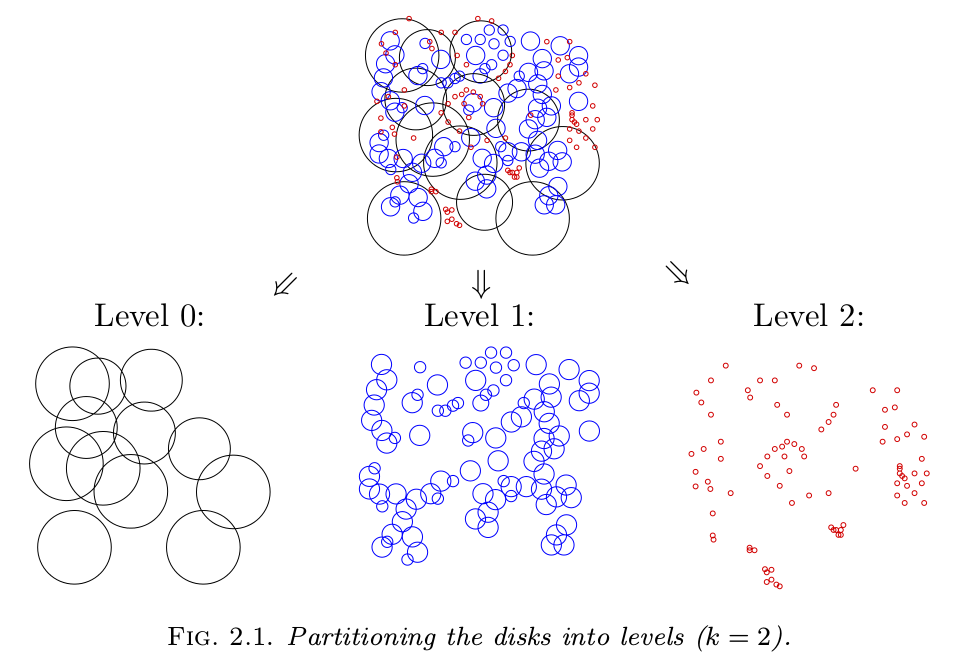
\includegraphics[width=1.0\textwidth]{img/2-1-fig.png}
      \end{figure}    
    \end{frame}
\/*
    \begin{frame}{}
      \begin{figure}[h!]
        \centering
          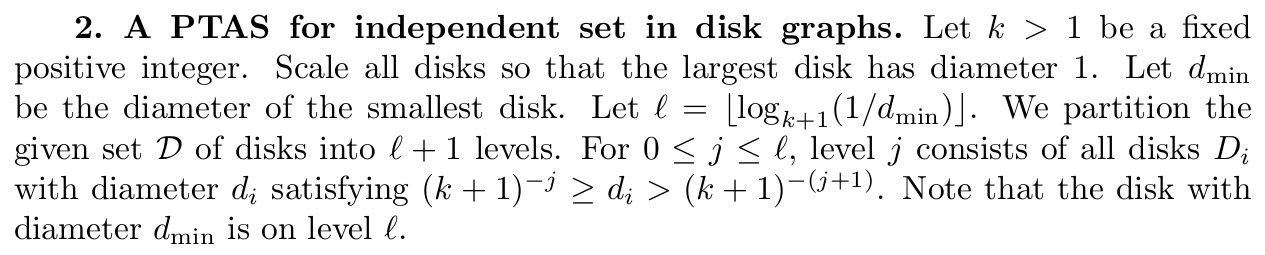
\includegraphics[width=1.0\textwidth]{img/model2.png}
      \end{figure}   
      \begin{figure}[h!]
        \centering
          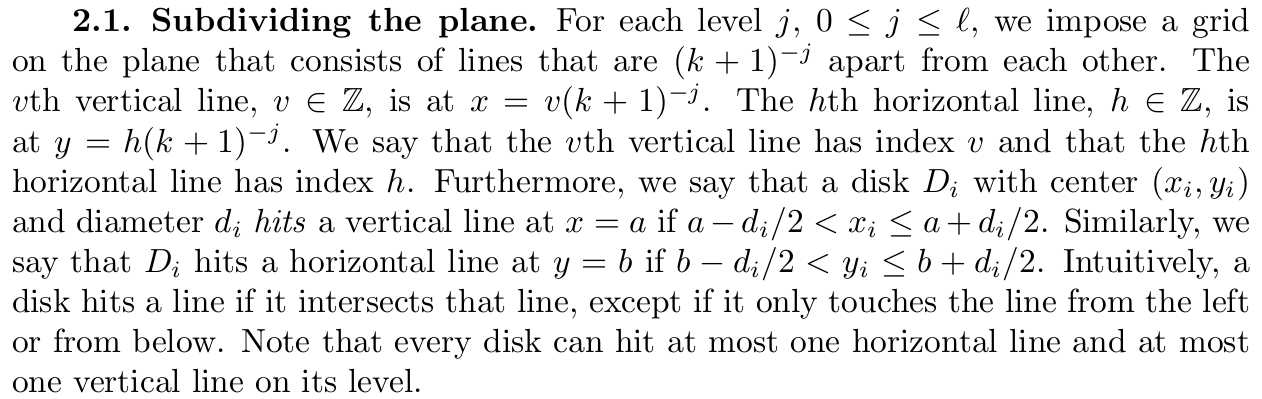
\includegraphics[width=1.0\textwidth]{img/model3.png}
      \end{figure}   
    \end{frame}

    \begin{frame}{}
      \begin{figure}[h!]
        \centering
          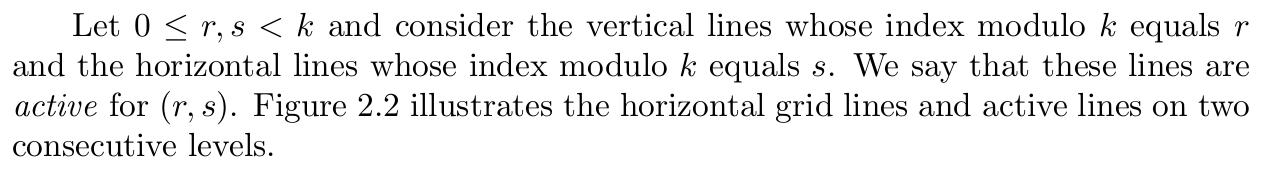
\includegraphics[width=1.0\textwidth]{img/model4.png}
      \end{figure}   
      \begin{figure}[h!]
        \centering
          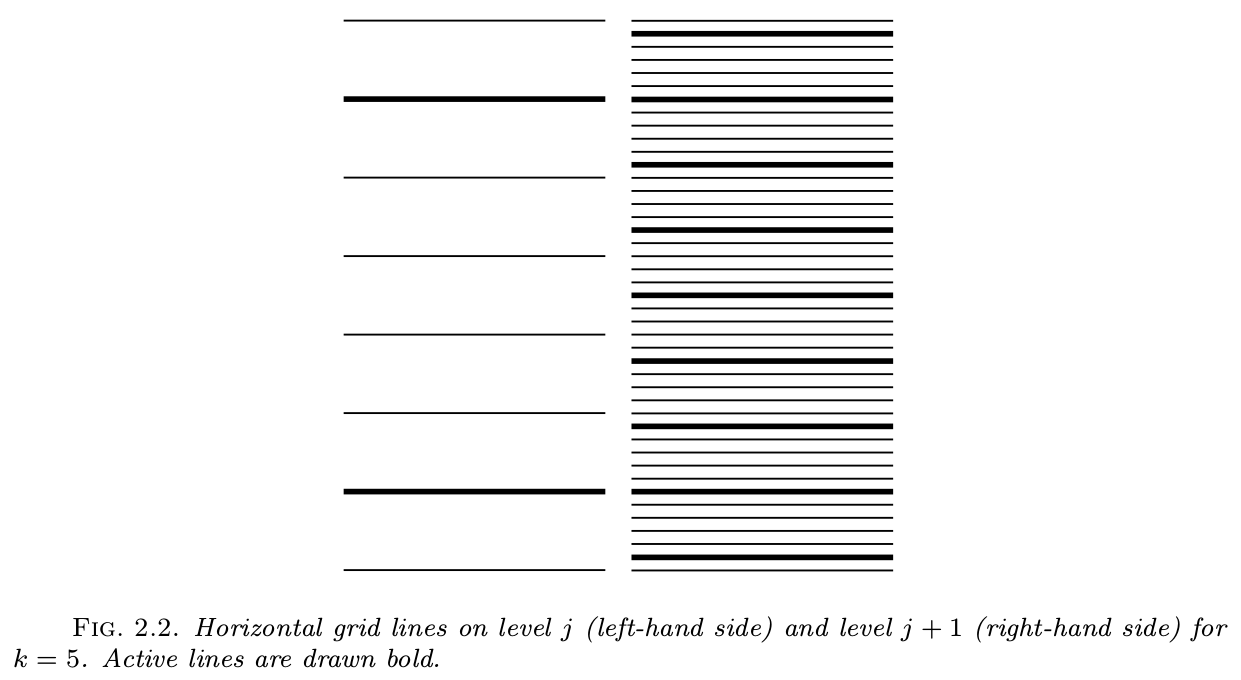
\includegraphics[width=1.0\textwidth]{img/2-2-fig.png}
      \end{figure}    
    \end{frame}

    \begin{frame}{}
      \begin{figure}[h!]
        \centering
          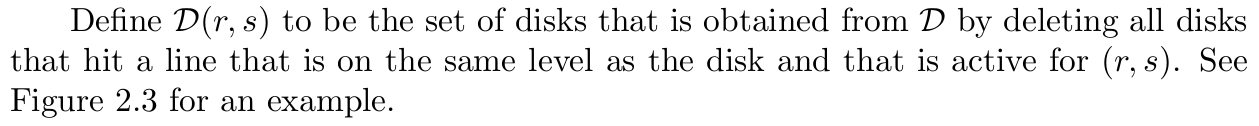
\includegraphics[width=1.0\textwidth]{img/model5.png}
      \end{figure}   
      \begin{figure}[h!]
        \centering
          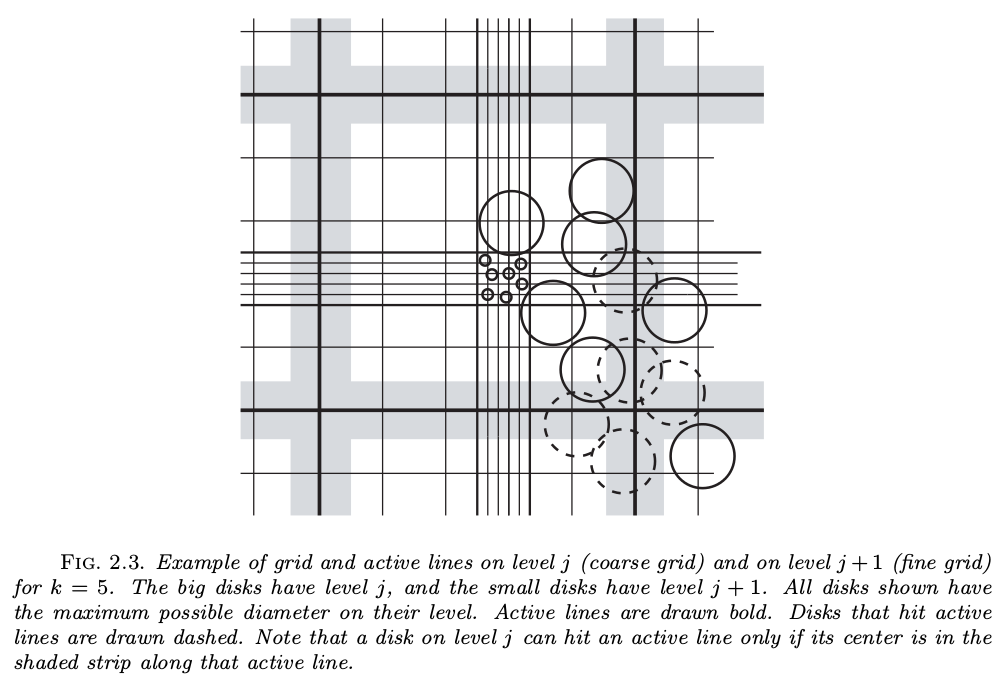
\includegraphics[width=0.8\textwidth]{img/2-3-fig.png}
      \end{figure}    
    \end{frame}
*/

  \section{Algorithm}
    \subsection{Overview}
      \begin{frame}{Divide and Conquer}
        \begin{figure}[h!]
          \centering
            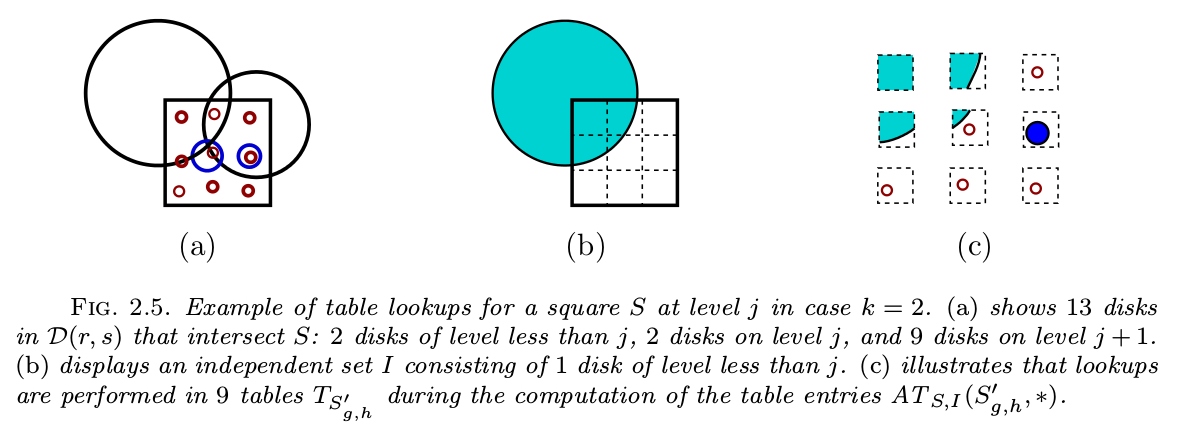
\includegraphics[width=1\textwidth]{img/2-5-fig.png}
        \end{figure}   
      \end{frame}

      \begin{frame}{Running-time}
        $$  \underbrace{ k^{2} \cdot n^{O(1)} }_{\tiny relevantSquare}
            \cdot (
            \underbrace{              
              \underbrace{ O(k^{2}) \cdot n^{O(k ^{2})} }_{\tiny missingTable}
              +             
              \underbrace{ n^{O(k ^{2})} }_{\tiny enumerateSet}
              \cdot
              \underbrace{ O(k^{2}) \cdot n^{O(k ^{2})} }_{\tiny computeAuxTable}
            }_{\tiny computeTable}
            )
        $$        
        \begin{block}{\small Procedures}
          \begin{description}
            \item[relevantSquare] {\small Compute relevant squares and their forest structure} \\
            \item[missingTable] Compute missing tables  $T_{S^{'}_{g,h}}$ \\
            \item[enumerateSet] {\small Enumerate sets $I$ for which $T_{S}(I)$ has to be computed } \\
            \item[computeAuxTable] Compute $AT_{S,I}()$ for each $S^{'}_{g_{1}..g_{2}, h_{1}..h_{2}}$ \\
          \end{description}
        \end{block}
      \end{frame}

    \subsection{Pseudo-Code}
      \begin{frame}{Dividing into Squares}
        \begin{figure}[h!]
          \centering
            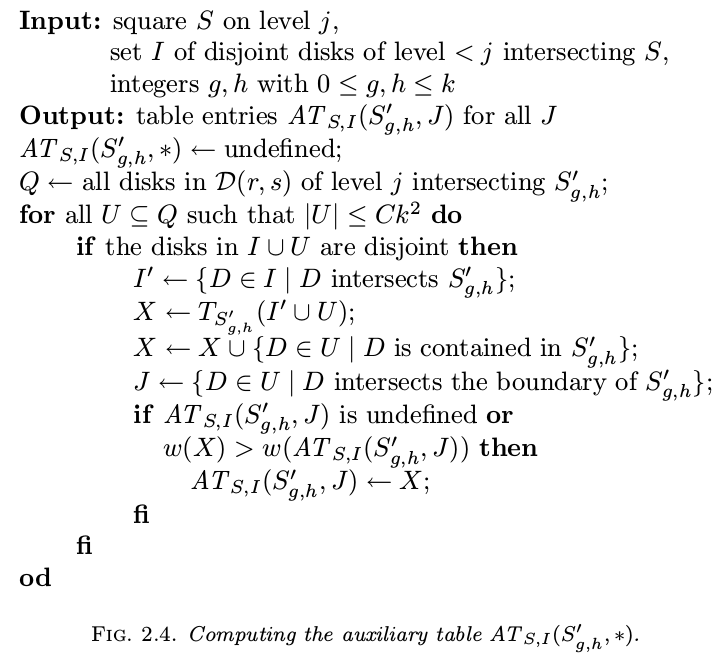
\includegraphics[width=0.7\textwidth]{img/2-4-fig.png}
        \end{figure}   
      \end{frame}
      \begin{frame}{Split}
        \begin{figure}[h!]
          \centering
            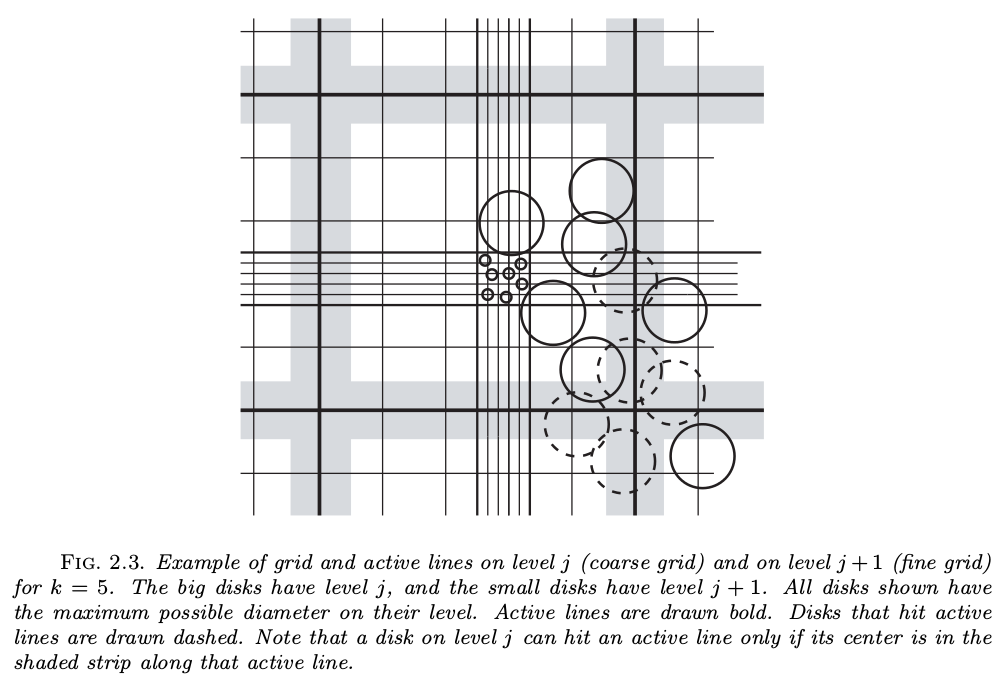
\includegraphics[width=0.9\textwidth]{img/2-3-fig.png}
        \end{figure}    
      \end{frame}

      \begin{frame}{Combining Rectangles}
        \begin{figure}[h!]
          \centering
            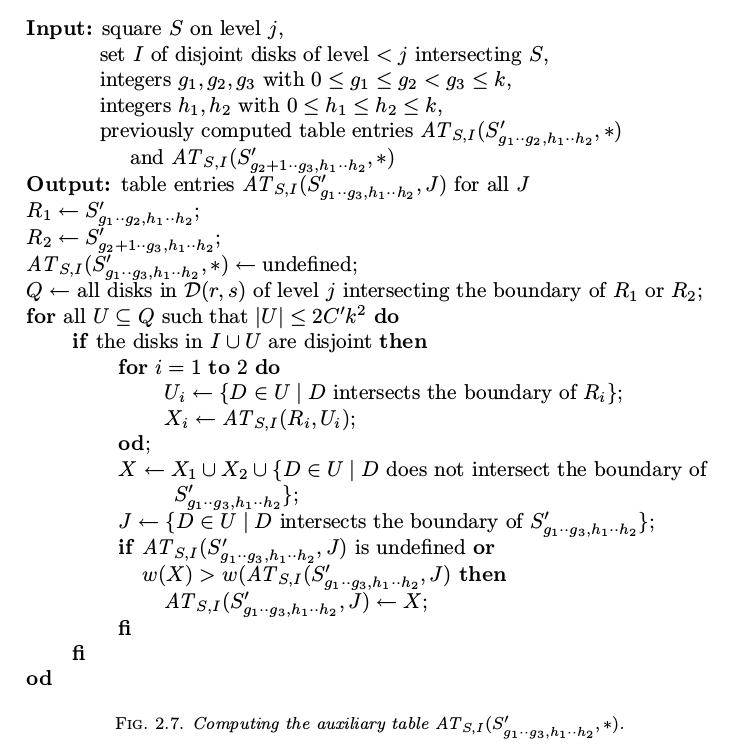
\includegraphics[width=0.65\textwidth]{img/2-7-fig.png}
        \end{figure}   
      \end{frame}        
      \begin{frame}{Merge}
        \begin{figure}[h!]
          \centering
            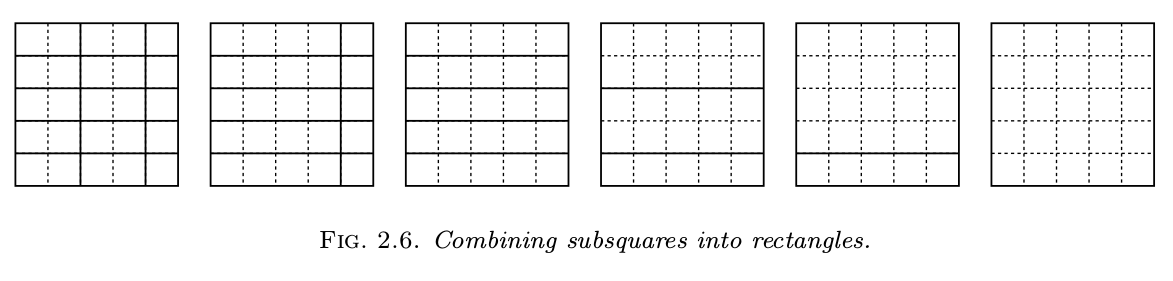
\includegraphics[width=1.0\textwidth]{img/2-6-fig.png}
        \end{figure}    
      \end{frame}

\/*
    \subsection{Procedures}
      \begin{frame}{Relevant Square}
        Call a $j$-square $S$ {\bf relevant} if $\mathcal{D}(r,s)$ contains at least one disk of level $j$ that is contained in $S$
        \begin{block}{j-square}
          \begin{figure}[h!]
            \centering
            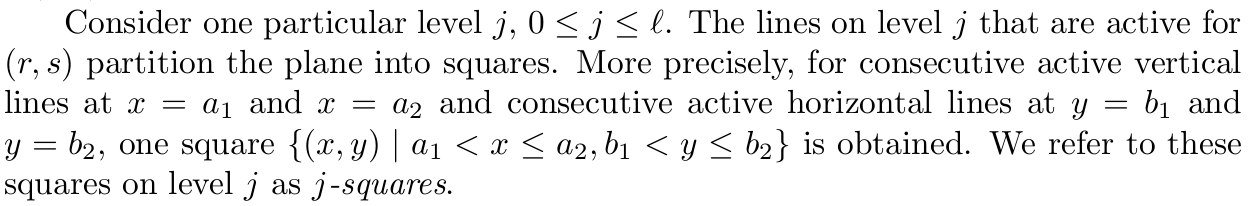
\includegraphics[width=1.0\textwidth]{img/j-square.png}
          \end{figure}
        \end{block}
      \end{frame}

      \begin{frame}{Missing Table}
        \begin{figure}[h!]
          \centering
          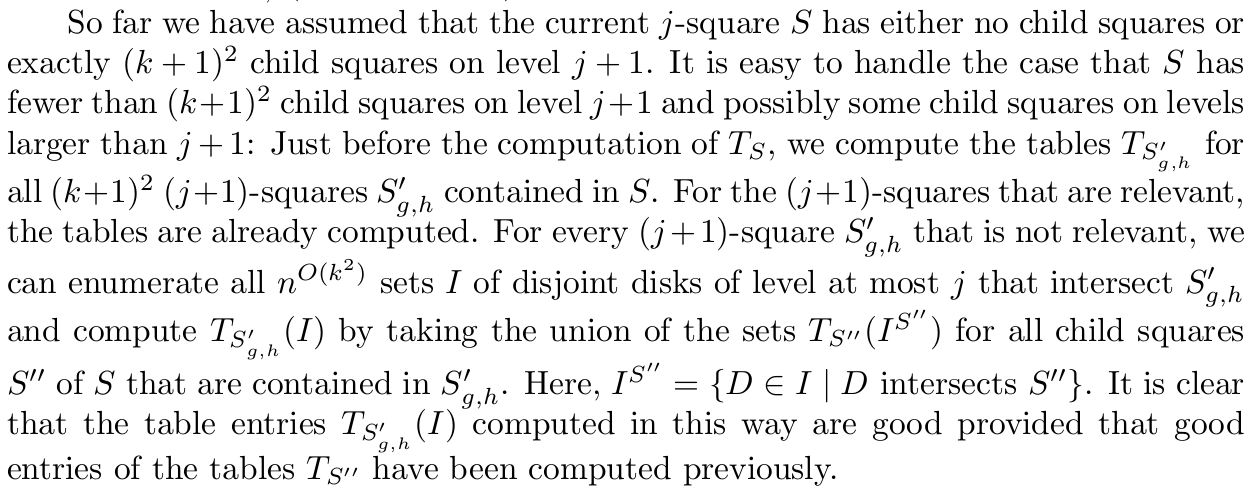
\includegraphics[width=1.0\textwidth]{img/missingTable.png}
        \end{figure}
      \end{frame}

      \begin{frame}{Compute $T_{S}(I)$}
        \begin{figure}[h!]
          \centering
          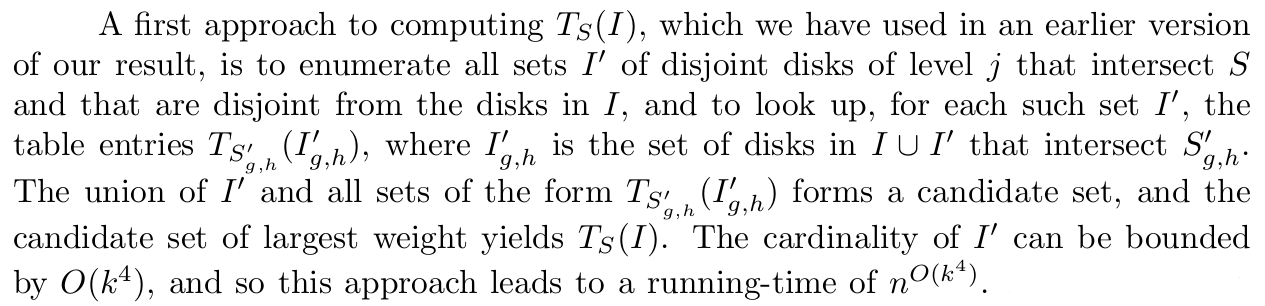
\includegraphics[width=1.0\textwidth]{img/computeTable-1.png}
        \end{figure}
      \end{frame}
      \begin{frame}{Enumerate sets $I$}
        \begin{figure}[h!]
          \centering
            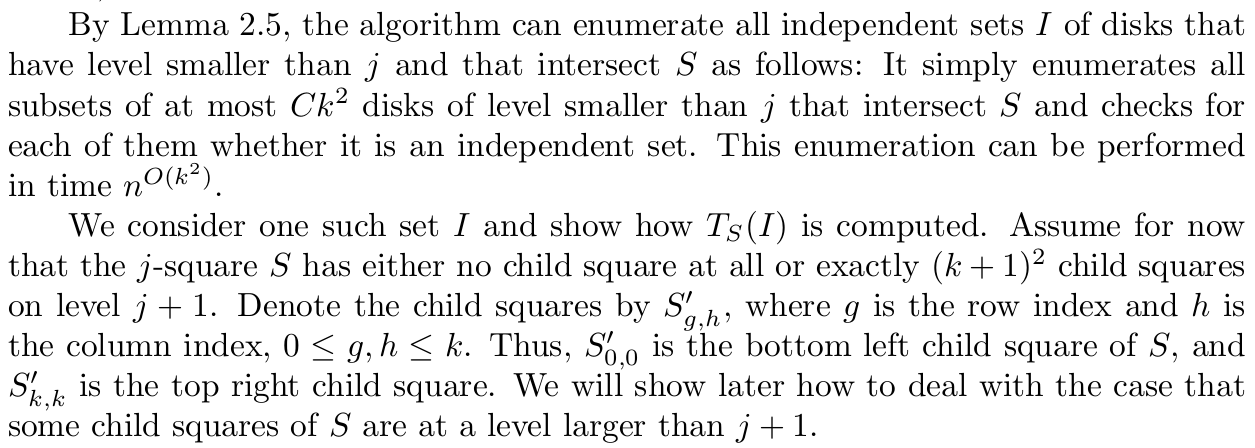
\includegraphics[width=1\textwidth]{img/enumerateSet.png}
        \end{figure}   
      \end{frame}

      \begin{frame}{Compute $T_{S}(I)$}
        \begin{figure}[h!]
          \centering
            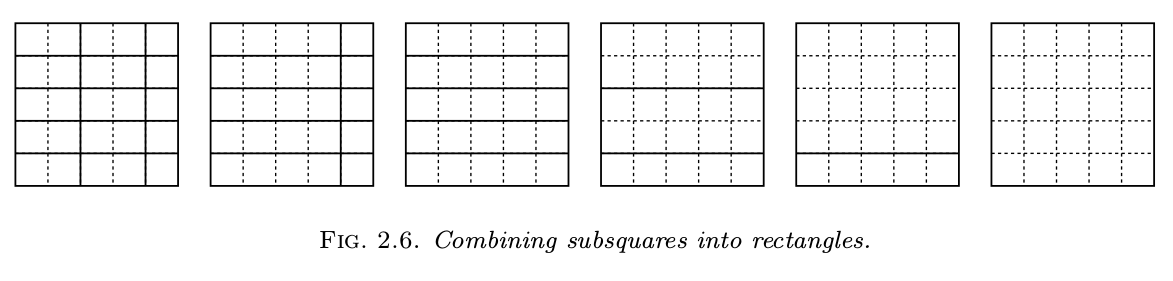
\includegraphics[width=1.0\textwidth]{img/2-6-fig.png}
        \end{figure}   
      \end{frame}
      \begin{frame}{Compute $T_{S}(I)$}
        \begin{figure}[h!]
          \centering
          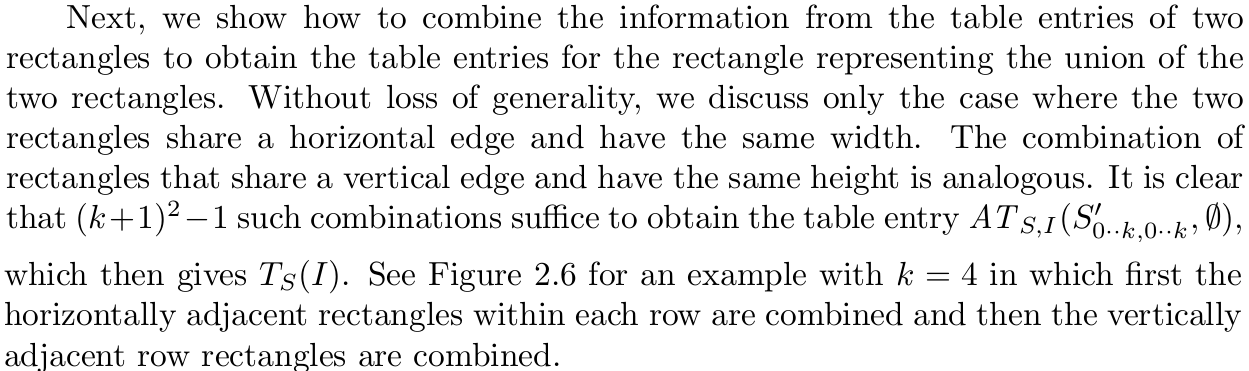
\includegraphics[width=1.0\textwidth]{img/computeTable-2.png}
        \end{figure}
      \end{frame}
      \begin{frame}{Compute $T_{S}(I)$}
        \begin{figure}[h!]
          \centering
            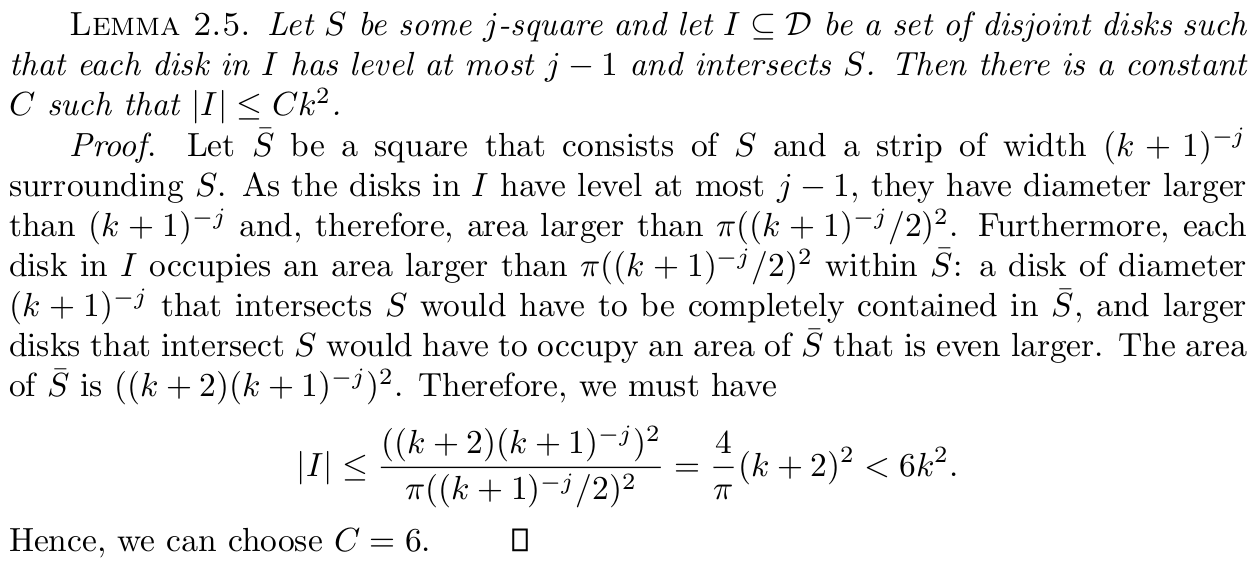
\includegraphics[width=1\textwidth]{img/2-5-lem.png}
        \end{figure}   
      \end{frame}

      \begin{frame}{Compute AT}
        \begin{figure}[h!]
          \centering
          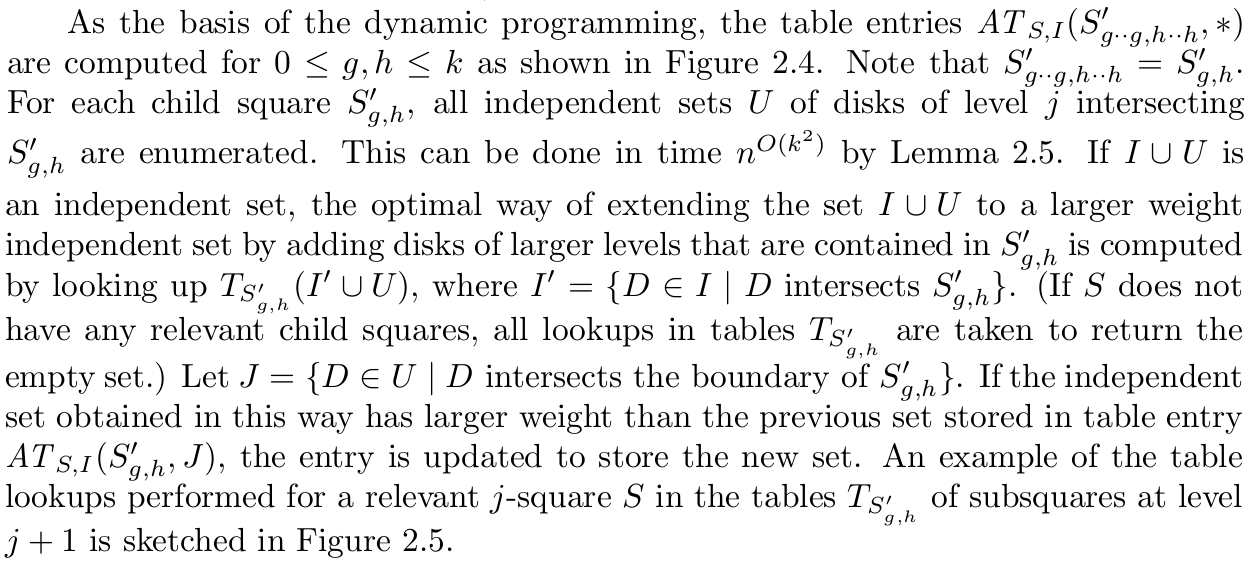
\includegraphics[width=1.0\textwidth]{img/computeAuxTable-1.png}
        \end{figure}
      \end{frame}
      \begin{frame}{Compute AT}      
        \begin{figure}[h!]
          \centering
            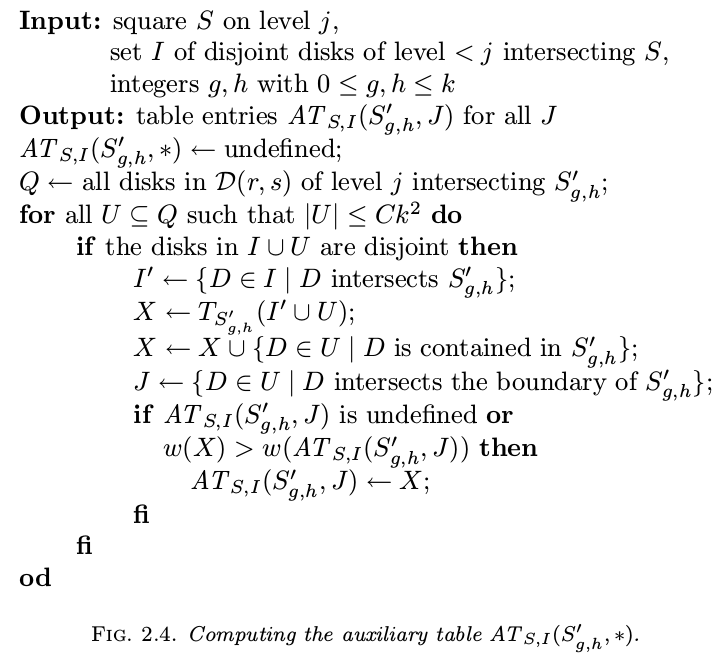
\includegraphics[width=0.75\textwidth]{img/2-4-fig.png}
        \end{figure}   
      \end{frame}
      \begin{frame}{Compute AT}      
        \begin{figure}[h!]
          \centering
            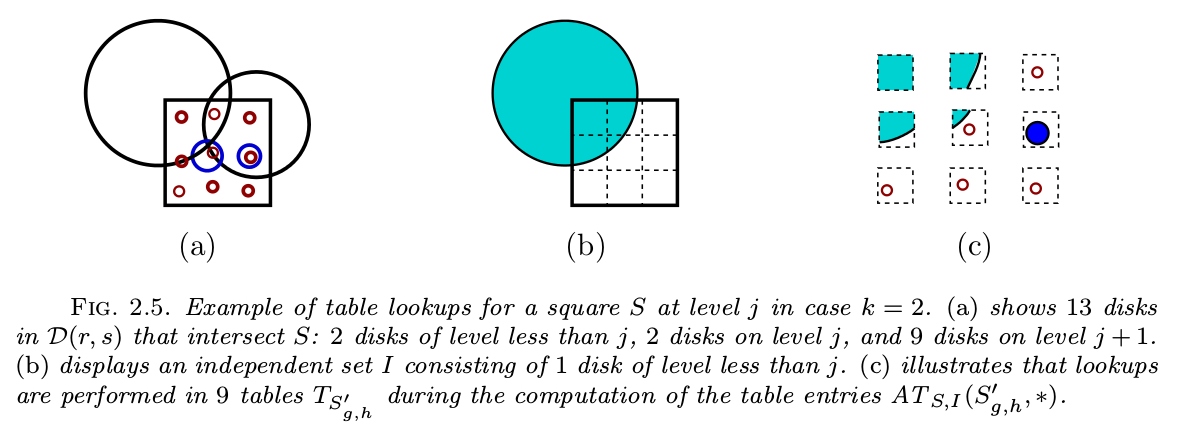
\includegraphics[width=1\textwidth]{img/2-5-fig.png}
        \end{figure}   
      \end{frame}
*/

    \subsection{Complexity}
      \begin{frame}{Running-time}
      \begin{block}{Polynomial for fixed $k>1$}
        $$  k^{2} \cdot n^{O(1)}
            \cdot \left(
            O(k^{2}) \cdot n^{O(k ^{2})}
            + 
            n^{O(k ^{2})}
            \cdot
            O(k^{2}) \cdot n^{O(k ^{2})} 
            \right)
            =            
            n^{O(k ^{2})}
        $$
      \end{block}
      \end{frame}


  \section{Approximation proof for the algorithm}

    \subsection{Lower bound}
      \begin{frame}{Subdividing the plane}
        \begin{figure}[h!]
          \centering
            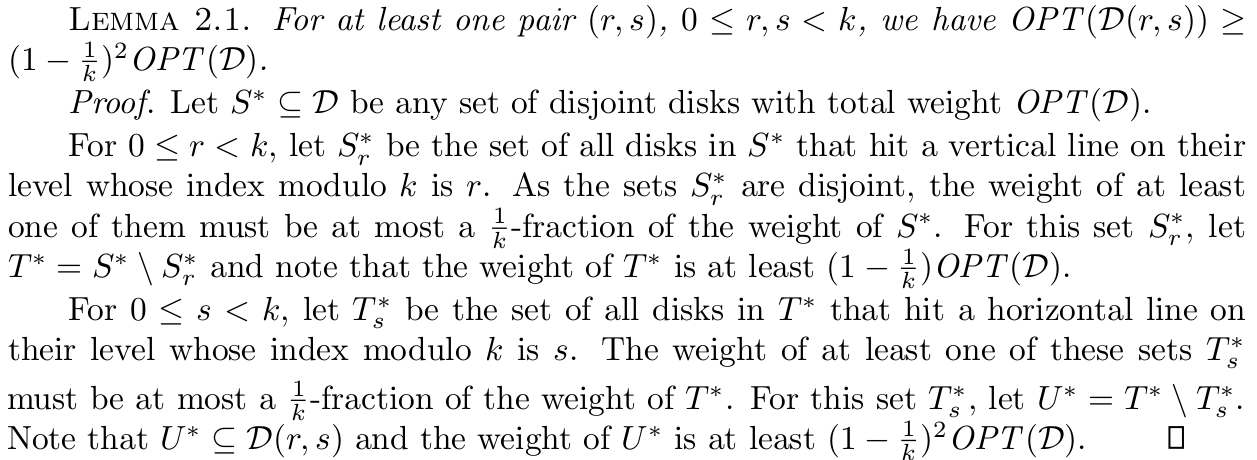
\includegraphics[width=1.0\textwidth]{img/2-1-lem.png}
        \end{figure}   
      \end{frame}

      \begin{frame}{$w(T^*) \geq \left( 1 - \frac{1}{k} \right) OPT(\mathcal{D})$}
        \begin{columns}
          \begin{column}{.5\linewidth}
            \begin{figure}[h!]
              \centering
                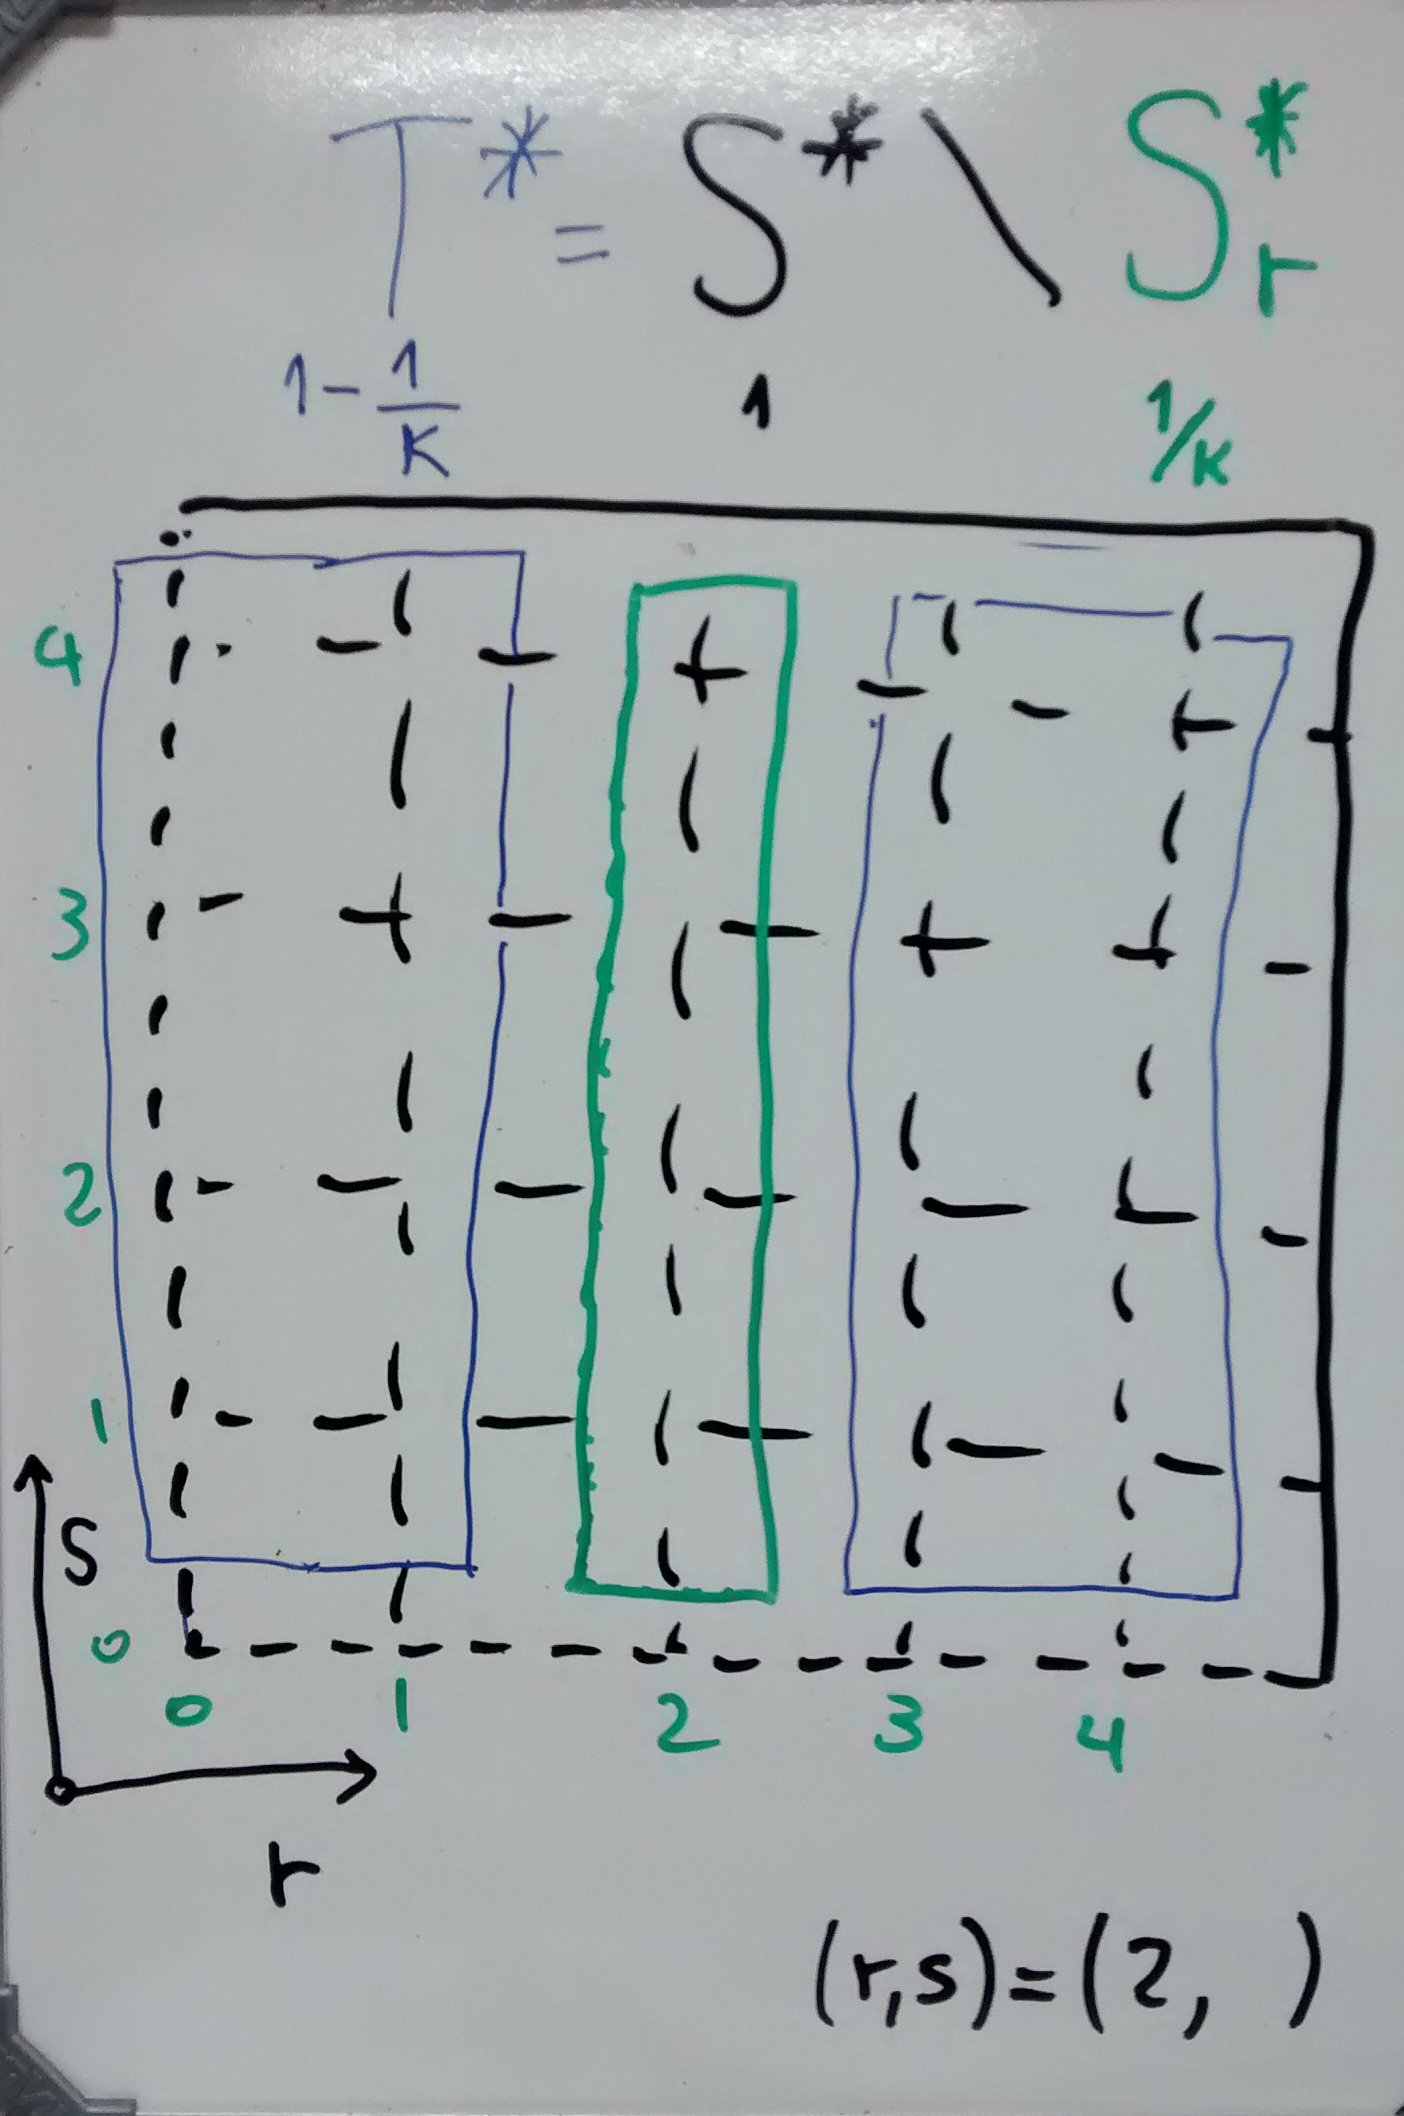
\includegraphics[width=0.8\textwidth]{img/2-1-lem-1.png}
            \end{figure}   
          \end{column}
          \begin{column}{.5\linewidth}
            \begin{block}{}
              Let $S^* \subseteq \mathcal{D}$ be any set of disjoint disks with total weight $OPT(\mathcal{D})$.
            \end{block}
            \begin{block}{}
              And $\mathcal{D}(r,s)$ defined as the set o disks that is obtained from $\mathcal{D}$ by deleting all disks that hit a line that is on the same level as the disk and that is active for $(r,s)$.
            \end{block}
          \end{column}
        \end{columns}
      \end{frame}

      \begin{frame}{ $U^* \subseteq \mathcal{D}(r,s)$ and $w(U^*) \geq \left( 1 - \frac{1}{k} \right)^2 OPT(\mathcal{D})$}
        \begin{columns}
          \begin{column}{.5\linewidth}
            \begin{figure}[h!]
              \centering
                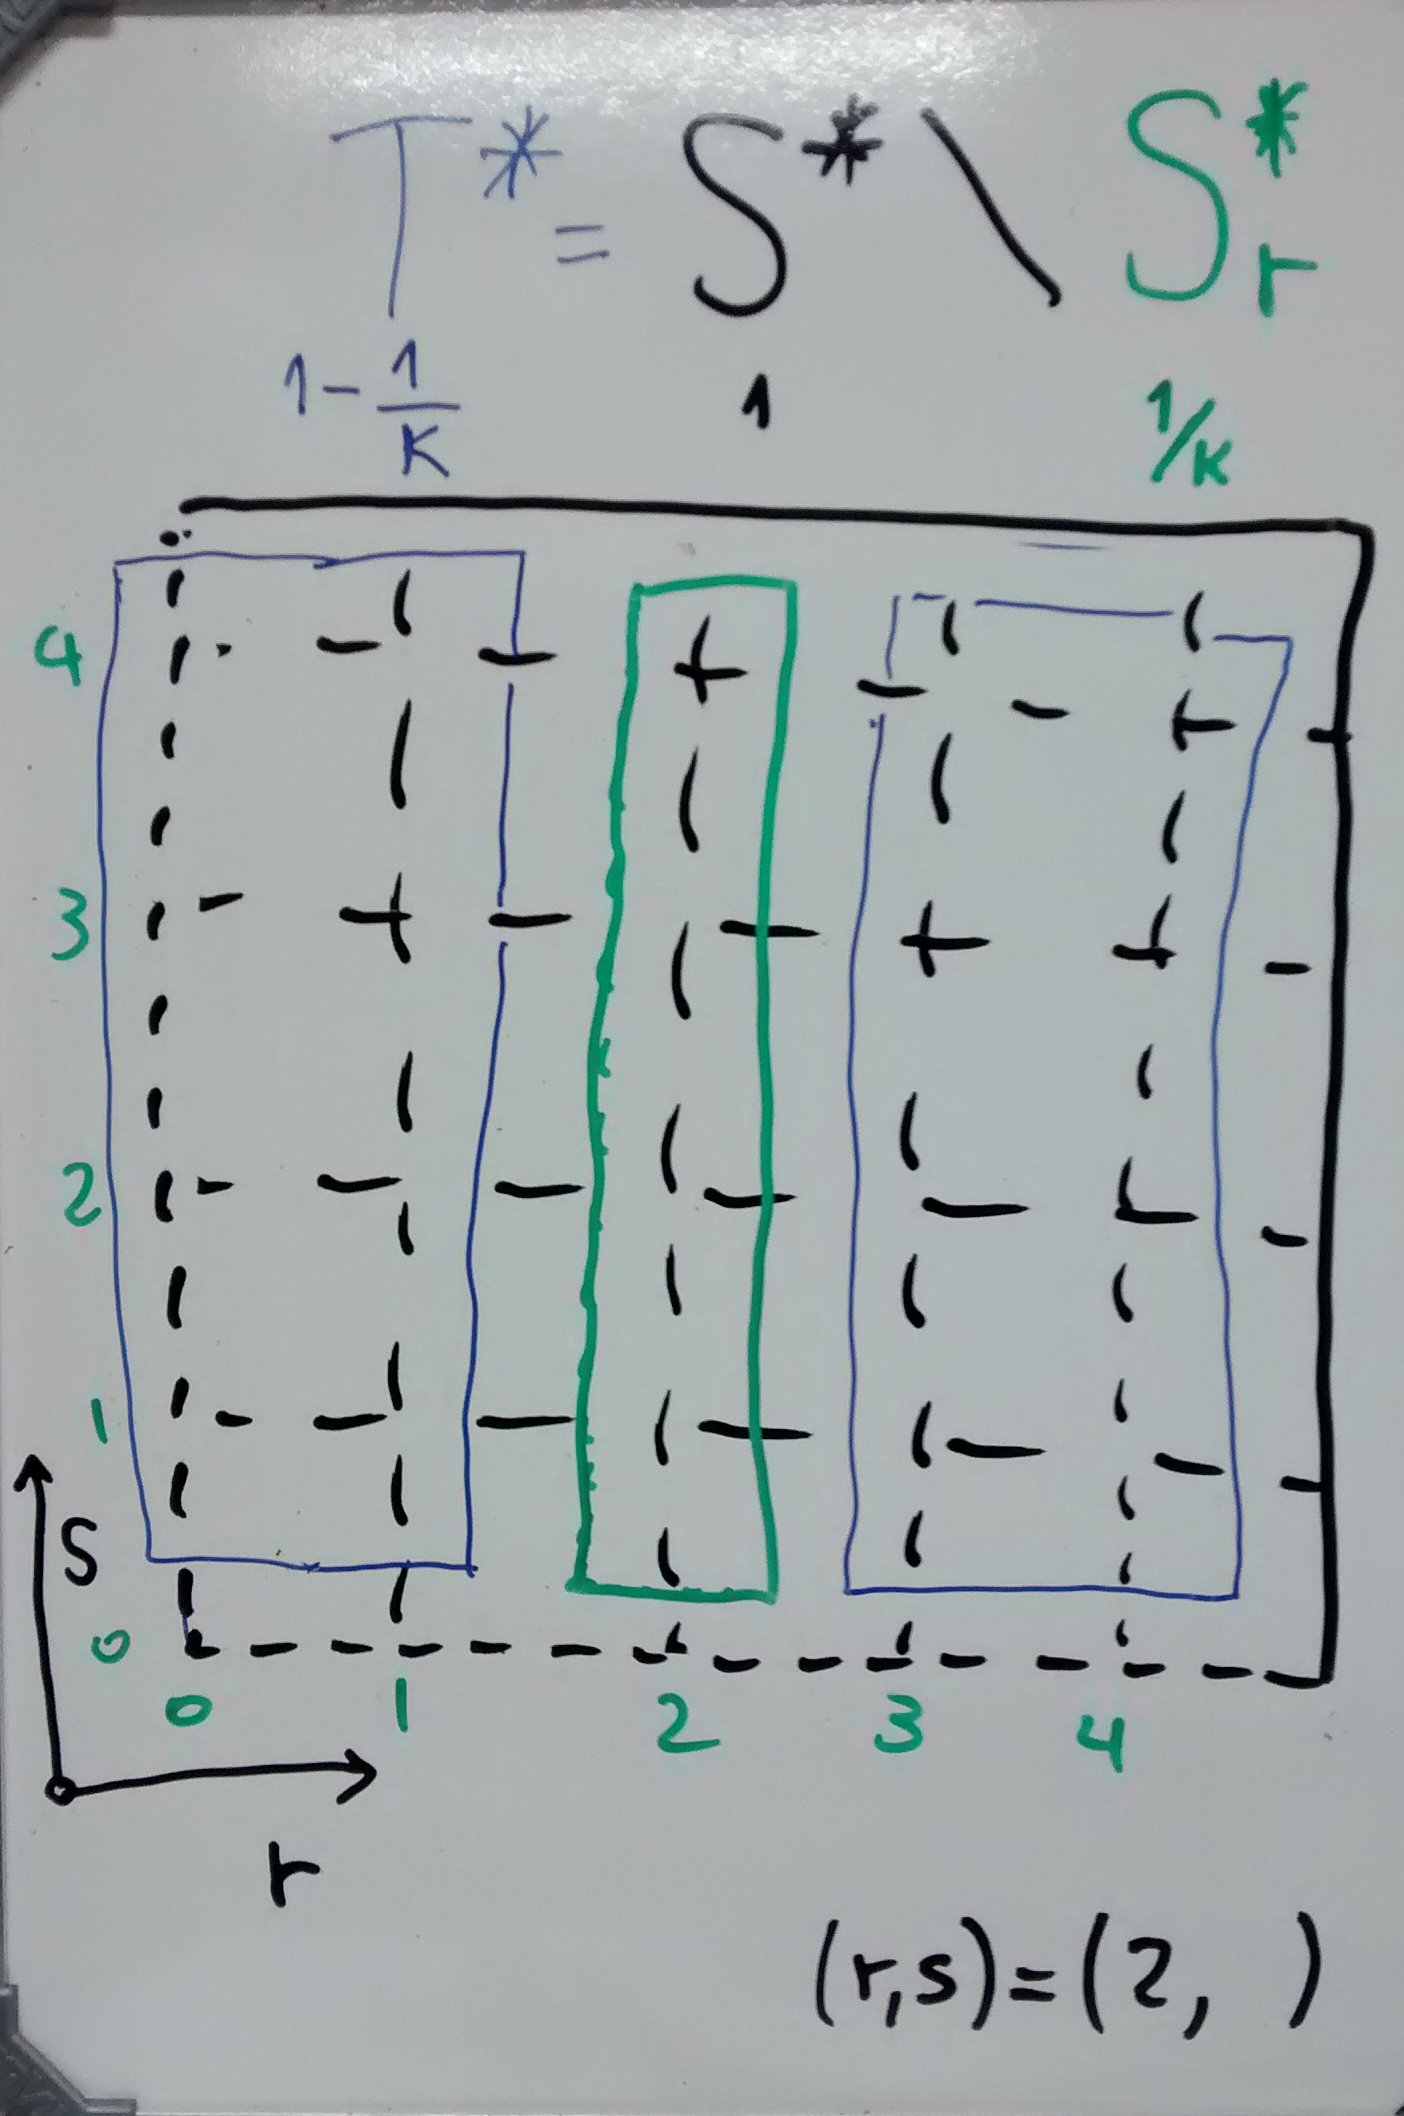
\includegraphics[width=0.6\textwidth]{img/2-1-lem-1.png}
            \end{figure}   
          \end{column}
          \begin{column}{.5\linewidth}
            \begin{figure}[h!]
              \centering
                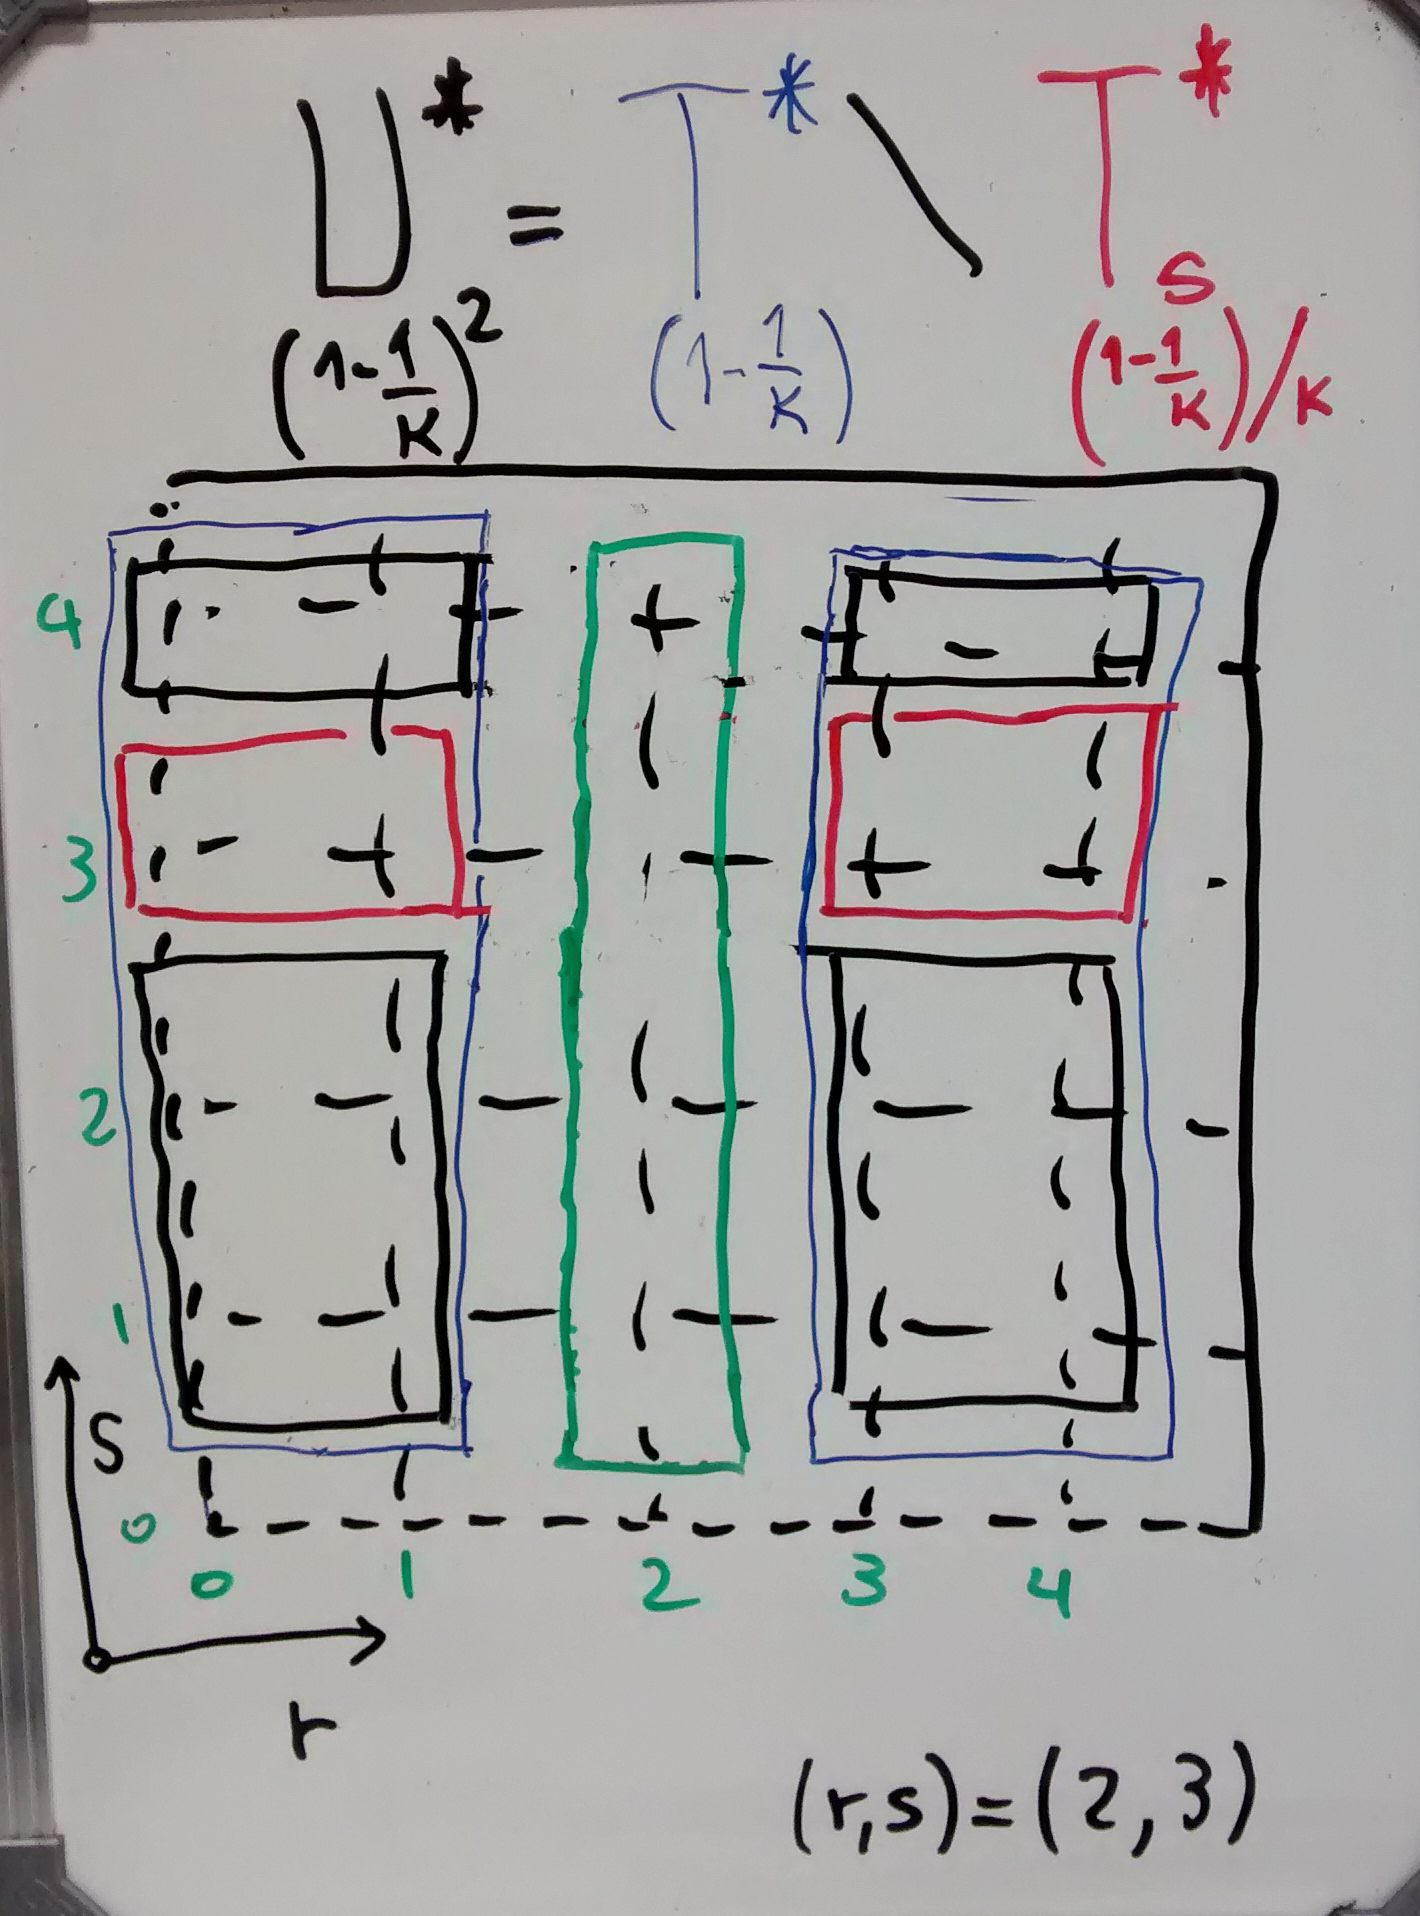
\includegraphics[width=0.9\textwidth]{img/2-1-lem-2.png}
            \end{figure}   
          \end{column}
        \end{columns}
      \end{frame}

      \begin{frame}{Approximation Ratio $\rho$}
        \begin{figure}[h!]
          \centering
            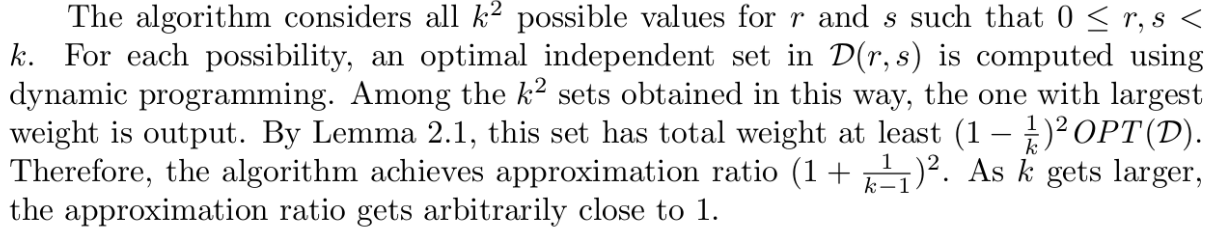
\includegraphics[width=1.0\textwidth]{img/upperBound.png}
        \end{figure}   
        $$\rho = \left(1 + \frac{1}{k-1}\right)^{2} \leq 1 + \frac{3}{k-1} = 1 + \epsilon$$
        $$\epsilon = \frac{3}{k-1}$$
      \end{frame}

      \begin{frame}{Running-time function of $\epsilon$}
        $$\epsilon = \frac{3}{k-1} \Rightarrow k = \ceil*{\frac{3}{\epsilon}}+1$$
        \begin{align*}
          \mbox{\Huge{$n^{O(k^2)} \Rightarrow n^{O\left(\frac{1}{\epsilon^{2}}\right)}$}}
        \end{align*}
      \end{frame}

    \subsection{Correcteness}

      \begin{frame}{An optimal independent set set can be computed}
        \begin{figure}[h!]
          \centering
            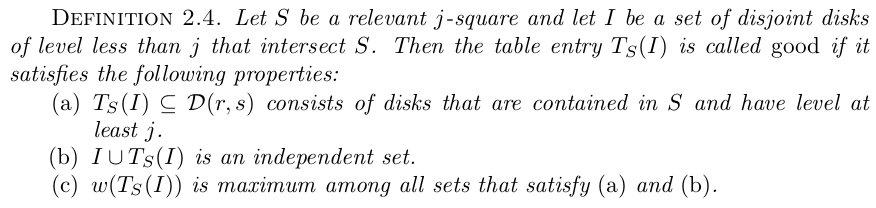
\includegraphics[width=0.9\textwidth]{img/2-4-def.png}
        \end{figure}   
        \begin{figure}[h!]
          \centering
            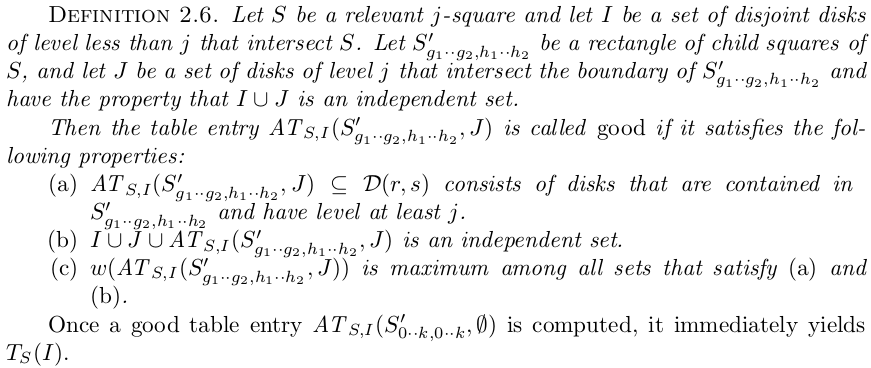
\includegraphics[width=0.9\textwidth]{img/2-6-def.png}
        \end{figure}   
      \end{frame}        

      \begin{frame}{Good Values}
        \begin{figure}[h!]
          \centering
            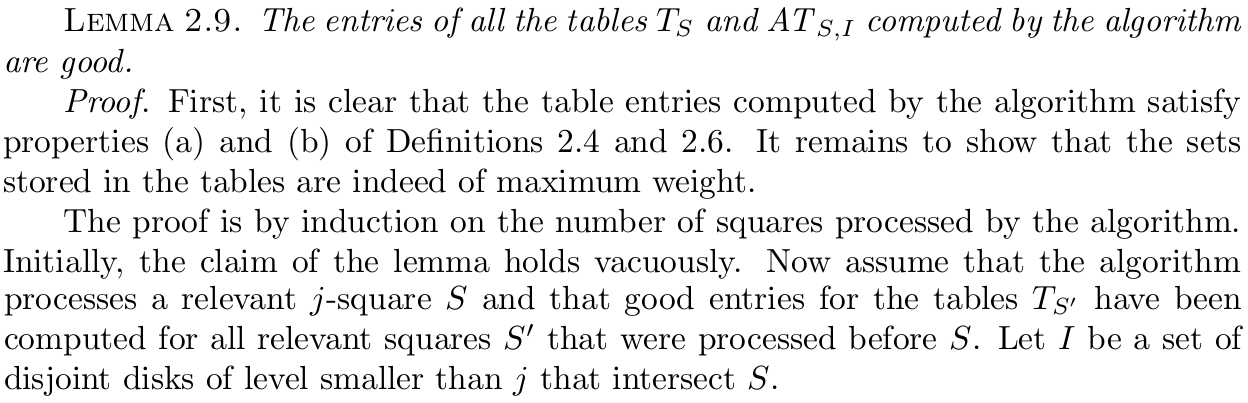
\includegraphics[width=1.0\textwidth]{img/2-9-lem-1.png}
        \end{figure}   
      \end{frame}        
      \begin{frame}{Map phase}
        \begin{figure}[h!]
          \centering
            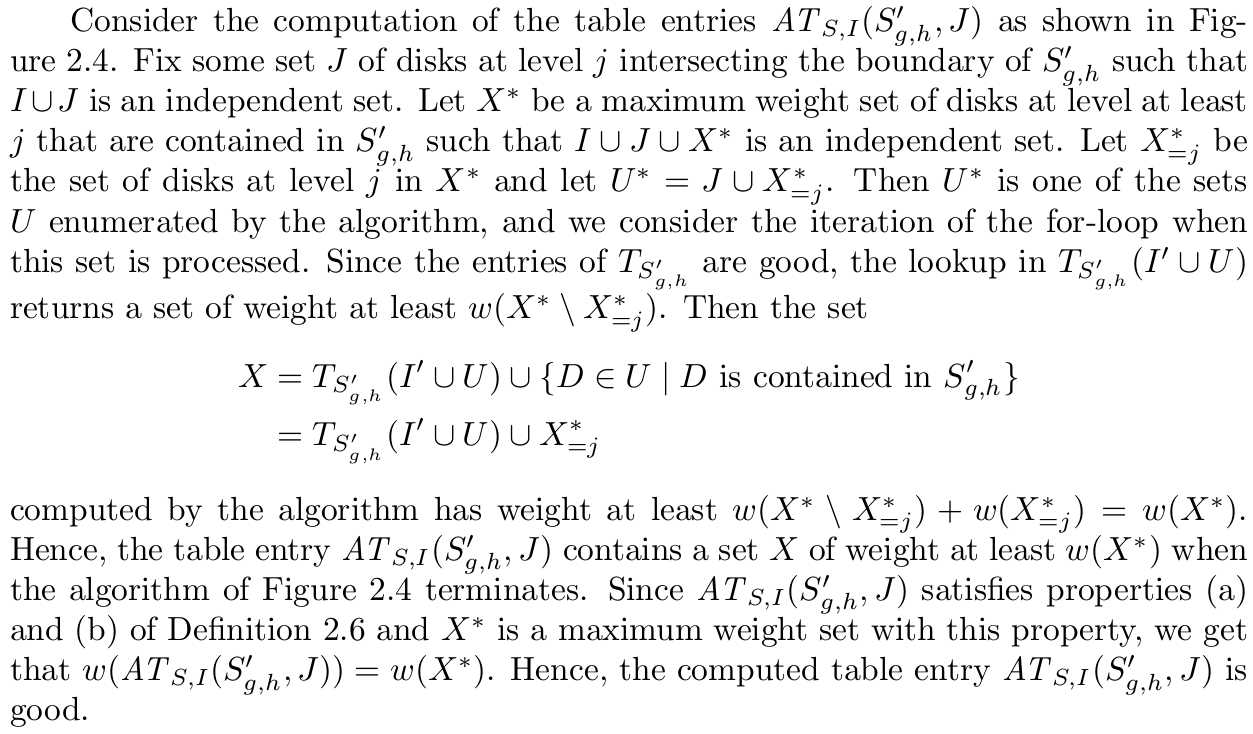
\includegraphics[width=1.0\textwidth]{img/2-9-lem-2.png}
        \end{figure}   
      \end{frame}        
      \begin{frame}{Reduce phase}
        \begin{figure}[h!]
          \centering
            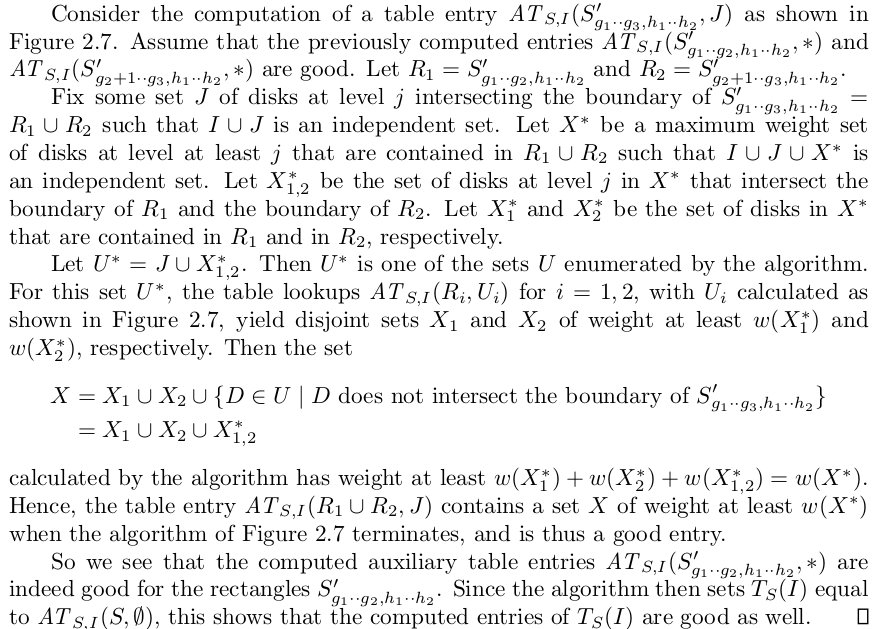
\includegraphics[width=0.9\textwidth]{img/2-9-lem-3.png}
        \end{figure}   
      \end{frame}

  \section{Conclusion}
    \subsection{MWIS PTAS}  
      \begin{frame}{Independent Set is 'not so' hard on disk graphs}
        \begin{block}{}
          There is a PTAS for MWIS in disk graphs,
          provided that a disk representation of the graph is given.
          The running-time for achieving approximation
          ratio $1 + \epsilon$ is $$n^{O\left(\frac{1}{\epsilon^{2}}\right)}$$ for a disk graph with $n$ disks.
        \end{block}
      \end{frame}    

    \subsection{Extension to $d$ dimensions}
      \begin{frame}{Independent Set is 'not so' hard on disk graphs and ...}
        \begin{block}{... the PTAS can be generalized to $d$ dimensions}
          There is a PTAS for MWIS in disk-like graphs,
          provided that a disk-like representation of the graph is given.
          The running-time for achieving approximation
          ratio $1 + \epsilon$ is $$n^{O\left(\frac{1}{\epsilon^{2(d-1)}}\right)}$$ for a disk-like graph with $n$ disk-like objects and any constant $d$.
        \end{block}
      \end{frame}    

  \section{}
    \subsection{}  
      \begin{frame}{Questions}
        \begin{figure}[h!]
          \centering
            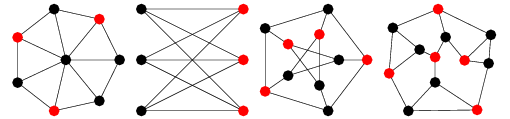
\includegraphics[width=0.5\textwidth]{img/mwis.png}
        \end{figure}
      \end{frame}    

  \section{}
    \subsection{}  
      \begin{frame}{Practical project - Possible approaches}
        \begin{enumerate}
          \item I will implement a simulation of the proposed algorithm and present an analysis of its performance in different scenarios and problems instances.
          \item And maybe, I will use the proposed algorithm to solve another problem.
        \end{enumerate}
      \end{frame}    

\end{document}
